\section{\SYSTEM{}: Combining Control and Learning}
\label{sec:framework}
A mobile device or embedded system runs a streaming application on a
heterogeneous processor.  We assume no prior knowledge of this
streaming application, but we do have prior knowledge of other
applications.  Our goal is to quickly build a model of the new
application and then control its resource usage such that it meets a
desired performance target with minimal energy.

\begin{figure}
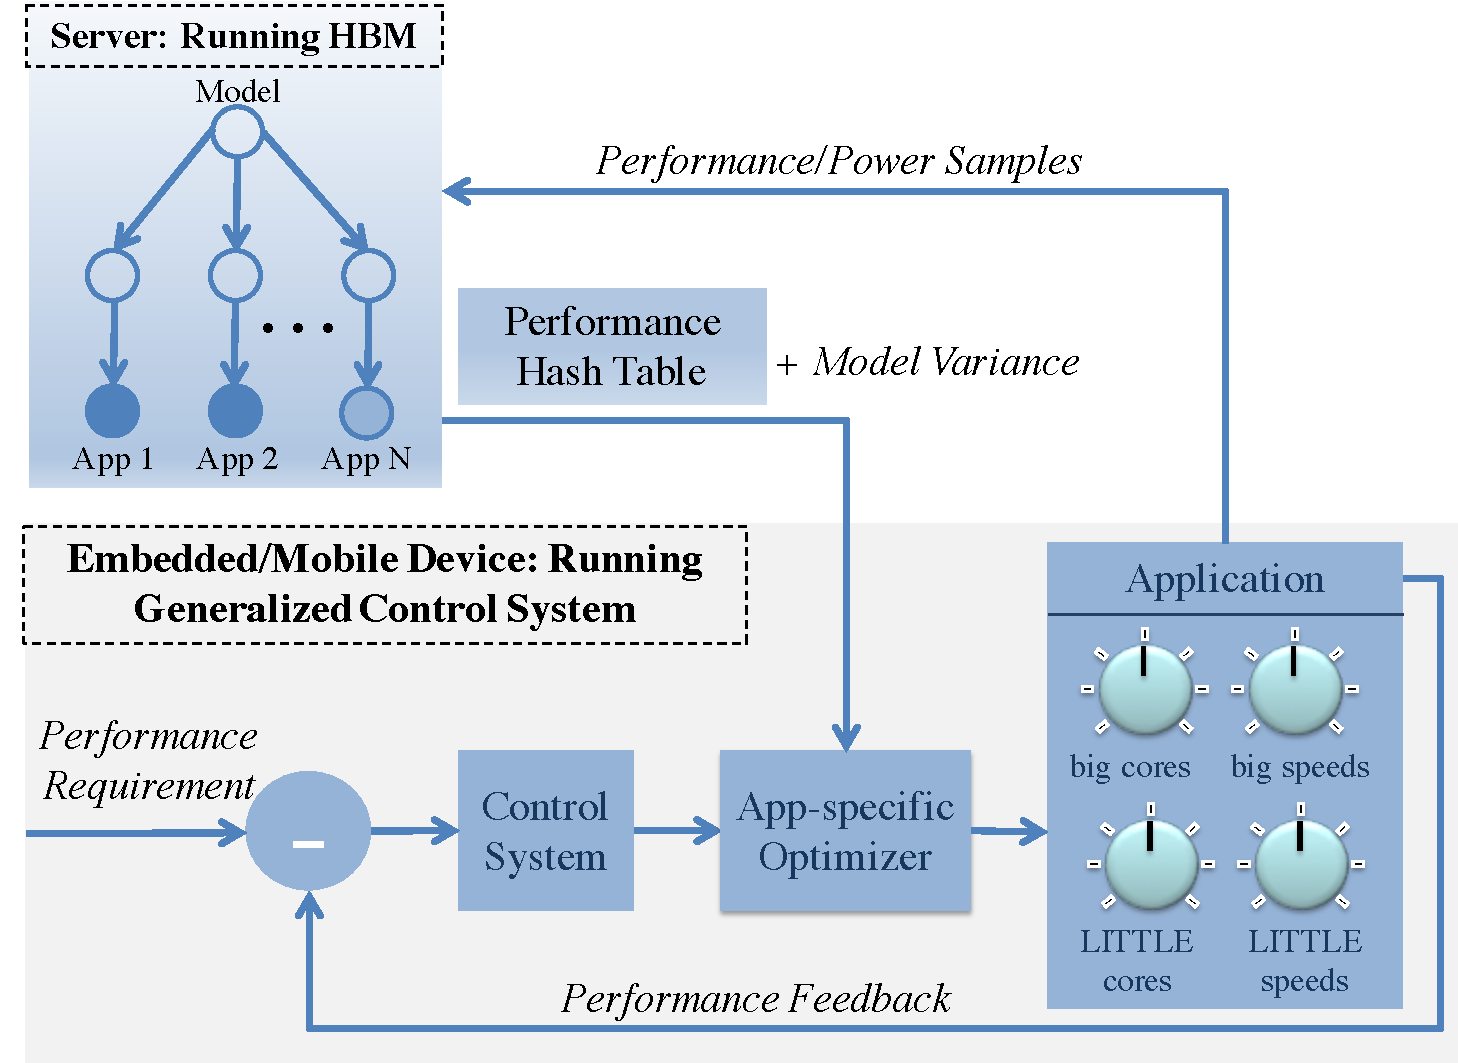
\includegraphics[width=\columnwidth]{figures/ControlLearning.pdf}
\caption{Overview of \SYSTEM{}.} 
\label{fig:overview}
\end{figure}

\figref{fig:overview} shows \SYSTEM{}'s approach to this problem.  On
the local device, a generalized control system (GCS) allocates
resources to the new application to meet its specified performance
goal with minimal energy.  The GCS starts with a generic resource
model, and as it selects configurations it records performance and
power in each configuration.  After recording a small number of values
(typically less than 10\% of the total configuration space).  These
recorded values are sent to a remote server which runs a hierarchical
Bayesian model (HBM).  The HBM estimates the application's performance
and power in all other configurations and extracts those
configurations that are Pareto-optimal in the performance/power
tradeoff space.  These configurations are packaged in a special data
structure -- the performance hash table (PHT) -- and sent to the GCS.
Using the PHT, the GCS selects an energy minimal resource
configuration in constant time ($O(1)$).  In addition to the PHT, the
server sends back the model's variance.  The GCS uses this variance to
customize control to the model's uncertainty, allowing guaranteed
convergence to the performance goal despite the fact that the system
starts with no prior knowledge of the streaming application.

The remainder of this section details \SYSTEM{}.  We begin by
describing a typical control design for a computer system and
illustrate how it fails to generalize.  We then describe \SYSTEM{}'s
generalized control system.  Next we discuss how \SYSTEM{} turns the
generalized control signal into specific resource configurations using
a model.  We then describe how to use a hierachical Bayesian model to
estimate resource performance and power tradeoffs.  We then describe
the performance hash table that encodes the learned model. We conclude
with some brief analysis of the approach, with detailed analysis
provided in an appendix.


\section{Traditional Control Design for Computing Systems}
A controller has a performance goal (corresponding to a
quality-of-service or real-time constraint) and adjusts system resource
usage to see that the goal is met.  In a simple example, a control
system might adjust processor frequency to ensure that a performance
goal is met \cite{lefurgy}.  Even better, an optimal controller would
use the minimal clockspeed to meet the performance requirement.

To turn clockspeed into performance a controller needs a model
relating these two values.  Directly mapping clockspeed to performance
is difficult -- a hypothetical model might account for instruction
mixes, memory hierarchy, memory latency, synchronization overheads,
etc.  Building such a model is tedious and error-prone process and
that is before we address system dynamics (\eg applications
transitioning from memory to compute bound).  Instead, control systems
use relatively simple difference models\footnote{Continuous time
  systems would use differential equations, but as time in computers
  is inherently discretized we restrict ourselves to discussion of
  difference equations which are appropriate for discrete time
  systems.}. 

%example difference model -- built into the controller
Continuing the example of controlling performance with clockspeed, a
simple model appropriate for control would be to assume that the
performance is a linear function of the clockspeed:
\begin{equation}
  perf(t) = k \cdot clock(t-1) + \delta \label{eqn:clock}
\end{equation}
Here, the observed performance $perf(t)$ is predicted as some constant
$k$ times the clockspeed applied at the previous time step,
$clock(t-1)$, plus some noise, $\delta$ drawn from a Gaussian
distribution.  This simple linear difference model ignores low-level
details like instruction mix, and instead uses feedback, predicting
behavior of the next time step as a function of the previous time
step.  Using the relationship of \eqnref{clock}, we can synthesize a
simple controller that is provably convergent to the desired
performance:
\begin{eqnarray}
  error(t) &=& goal - perf(t) \label{eqn:clock-error} \\
  clock(t) &=& clock(t-1) - \frac{error(t)}{k}
  \label{eqn:clock-control}
\end{eqnarray}


% Can we make the model a tunable parameter?
The controller of \eqnref{clock-control} provides formal guarantees
that it will converge to the desired performance ($goal$ in
\eqnref{clock-error}) and it bounds the time taken to converge.  All
these guarantees, however, are predicated on the accuracy of the
model; \ie on the value $k$ in this simple example.  This value is
highly dependent on the particular application under control.  More
complicated examples that control multiple resources are relatively
straightforward extensions of the example shown here that use matrix
equations instead of the scalar equations presented here
\cite{METE,others}.  Either way, the control system is highly
dependent on the value of $k$ -- we could set $k$ to be
application specific, but that controller will fail on some
applications.  If we choose a value of $k$ such that performance still
converges to the goal for all applications it will be very slow,
meaning that the controller will take many time steps to react to some
dynamic events.  It would clearly be beneficial to tune the control
models to individual applications.

\section{Generalized Control Design}
We would like to use control and learning to solve the problem of
meeting an application's performance requirements while minimizing
energy consumption.  The difficulty is that classical control
formulations like the example above integrate the models directly into
the controller; \ie the application-dependent relationship between
performance and resource usage is directly used in the control
equations.  We propose to address this problem using the classic
computer science trick of adding a layer of indirection.  This idea is
illustrated in \figref{overview}.  Instead of directly controlling
resources using an application-dependent model, we will control
\emph{speedup} and pass that speedup value to a separate module that
translates speedup into a desired resource configuration using the
learned models.  In this section, we first describe our formulation
for controlling speedup and then describe the translator that converts
that speedup into resource allocations.

\subsubsection{Controlling Speedup}
Analogous to \eqnref{clock} we write a simple difference model
relating speedup to performance:
\begin{equation}
  perf(t) = b \cdot speedup(t-1) + \delta \label{eqn:speedup}
\end{equation}
where $b$ is the \emph{base speed} of the application, here defined as
the speed when all resources are available.  While $b$ is application
specific, it is easy to measure online, by simply allocating all
resources. Such a configuration should not violate any performance
constraints (although it is unlikely to be energy efficient) so it is
safe to take this measurement without risk of violating performance
constraints.

With this model, the control law is simply:
\begin{eqnarray}
  error(t) &=& goal - perf(t) \label{eqn:speedup-error} \\
  speedup(t) &=& speedup(t-1) - \frac{error(t)}{b}
  \label{eqn:speedup-control}
\end{eqnarray}
which states that the speedup to apply at time $t$ is a function of
the previous speedup, the error at time $t$ and the base speed $b$.
This is a very simple \emph{deadbeat} \TODO{need to add a pole -- so
  it will no longer be a deadbeat controller} controller that provides
all the standard control theoretic formal guarantees.  By measuring
base speed online while the application runs, we can tune the control
to a specific application.  We note that using this definition of base
speed, most speedups will be less than one.  In addition to making
base speed easier to measure, this has the nice property of bounding
the learner's output, making for more robust learning \TODO{Nikita,
  what am I trying to say here? Or should we just put a forward
  reference because the next section benefits from a max speedup of 1}
Of course, we still have the challenging problem of converting an
abstract speedup into an actual resource allocation.


\section{Allocating Resources with a General Control Signal}
We need to map the speedup produced by \eqnref{speedup-control} into a
resource allocation.  On our target system, an ARM big.LITTLE
architecture, that specifically means mapping speedup into a number of
big cores, a number of small cores, and a speed for both (on our
system big and little cores can be clocked separately).

The primary challenge here is that the HBM produces a discrete
non-linear function of resource usage into speedup and powerup, while
\eqnref{speedup-control} is a continuous linear function.  We bridge
this divide by assigning time to resource allocations such that the
average speedup over a control interval is that produced by
\eqnref{speedup-control}.

We call an assignment of time to resources a schedule.  Not
surprisingly, there are typically many schedules that meet a
particular performance requirement.  We would like to find a minimal
energy schedule. Given a time interval $\tau$, a workload $W$ to
complete in that interval, and a set of $C$ configurations, we
formalize this problem as:
\begin{eqnarray}
  \minimize && \sum_{c=0}^{C-1} \tau_c \cdot p_c \label{eqn:power} \\
  \st %&& \nonumber\\
  && \sum_{c=0}^{C-1} \tau_c \cdot s_c \cdot b =  W \label{eqn:work} \\
  && \sum_{c=0}^{C-1} \tau_c =  \tau \label{eqn:deadline} \\
  && 0 \le \tau_c \le \tau, \qquad \forall c \in \{0,\ldots,C-1\} \label{eqn:time}
\end{eqnarray}
where $p_c$ and $s_c$ are the estimated powerup and speedup of
configuration $c$ and $\tau_c$ is the amount of time to spend in
configuration $c$.  \eqnref{power} simply states that the objective is
to minimize energy (power times time).  \eqnref{work} states that the
work must be done, while \eqnref{deadline} requires the work to be
done on time.  \eqnref{time} simply avoids negative time.  


\section{Learning Power/Performance Tradeoffs}


\section{Encoding Learned Models}


\section{Analysis}
\TODO{This needs to be brief, and we can put any details in an
  appendix.}

\subsection{Algorithmic Analysis}

\subsubsection{Control System Complexity}

\subsubsection{Learning System Complexity}

\subsection{Control Theoretic Formal Guarantees}
